\documentclass[conference]{IEEEtran}
\IEEEoverridecommandlockouts
% The preceding line is only needed to identify funding in the first footnote. If that is unneeded, please comment it out.
\usepackage{cite}
\usepackage{amsmath,amssymb,amsfonts}
\usepackage{algorithmic}
\usepackage{graphicx}
\usepackage{textcomp}
\usepackage{xcolor}
\usepackage{hyperref}


\def\BibTeX{{\rm B\kern-.05em{\sc i\kern-.025em b}\kern-.08em
    T\kern-.1667em\lower.7ex\hbox{E}\kern-.125emX}}
\begin{document}

\title{
\includegraphics[scale=0.4]{IST.png} \\ \vspace{30px} 
\includegraphics[scale=0.06]{../Immersivaudio logo.png} \\Immersivaudio: audio generation based on video features.}

\author{\IEEEauthorblockN{Michele Vitale}
\IEEEauthorblockA{\textit{ist1111558}}
\and
\IEEEauthorblockN{Daniele Avolio}
\IEEEauthorblockA{\textit{ist1111559}}
\and
\IEEEauthorblockN{Teodor Chakarov}
\IEEEauthorblockA{\textit{ist1111601}}
}

\maketitle
 
\section{Introduction}
Generative Artificial Intelligence has brought a completely new approach to the process of creating digital contents: since the public release of services such as ChatGPT \cite{chatgptintro} or DALL-E \cite{dall-e}, the field has been growing exponentially, with new models and applications that can produce text, images, audio and even videos with growing quality levels.
\\In this project we deepen some of the tasks and possibilities that these models can offer, with the aim of using state-of-art models that are freely available to the public to solve a multimedia task.

\section{Problem description}
The problem we are trying to solve is the enhancement of a video by adding an audio track that can better fit the content of the video itself. The audio track can be both music or music and sound effects, based on the user preferences. \\
The problem can fit in various scenarios and contexts, such the creation of audio for a video that has to be published on social medias and requires copyright-free music (it might be the case of online platforms such as YouTube, where the copyright policies are very strict \cite{ytcopyright}), visually impaired people that can get a more immersive experience from a video combining our solution with already existing audio description services, or simply to enhance audio tracks of videos that have noisy or low-quality audio or that have no audio at all, such as drones footage or submarine recordings. \\
Thus, the range of use cases of the system is wide and flexibility is a key requirement. 

\section{Proposed solution}
The proposed solution is a pipeline that takes in input a video and returns the input video combined with the enhanced audio track. It is composed of a number of modules that decompose the problem into clear and manageable tasks, with the idea of making the system modular, scalable, easily adaptable to different scenarios and deployable on various workload distribution models, such as computer or container clusters. \\
The main idea is to use the features of the video to generate a prompt that can be used to condition the audio generation module, so that the generated audio can better fit the video. The features of the video extracted during the process are based on the content of a number of frames extracted by the input. Each step of the process has been discussed in the following sections, in particular in the \textbf{Architecture} section of this report.

\section{Architecture}

\begin{figure}[h]
    \centerline{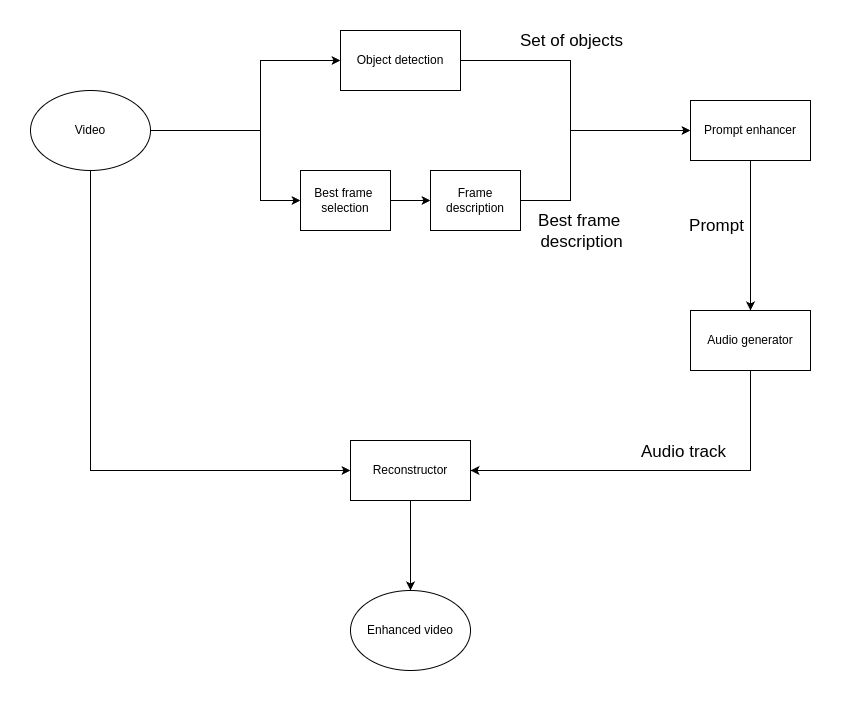
\includegraphics[width=0.5\textwidth]{final_architecture.png}}
    \caption{Architecture of the system.}
    \label{architecture}
\end{figure}
The complete architecture of the system is shown in Figure \ref{architecture}.
The figure shows the architecture of the whole pipeline applied to a video,
but other pipelines are provided to adapt to different use cases and input types.
The different components of the system are communicating using the JSON format and each module is appending its output rather than reshaping the output to be only the required one from the following step, enabling the process to be modular and adaptable to different scenarios.\\
Each video is internally identified with an unique token, which is computed at input as the MD5 hash of the video itself. 
The Input/Output process is made using the Gradio \cite{Gradio} library, which allows the fast development of GUIs, especially for machine learning models. The GUIs are served on a simple web interface.
 
\subsection{Frame extraction}
The frame extraction module takes in input a video and extracts a number of frames. 
Not every frame in the video is used, because it would be computationally expensive and not necessary since close frames usually have similar features and objects.\\
The initial idea to sample frames was to fix a specific number for each second of the video, 
but this approach was discarded due to the increasing amount of frames for longer videos. The final approach used in the project is to sample a number of frames based on a function of the input length video, specifically:
$$n = k \cdot log_{10}(s)$$
with $n$ being the number of frames, $s$ the length of the video in seconds and $k$ a constant factor given in input. This approach was chosen to have a logarithmic growth of the number of frames, which is more computationally efficient and still provides a good representation of the video.\\
\begin{figure}[h]
    \centerline{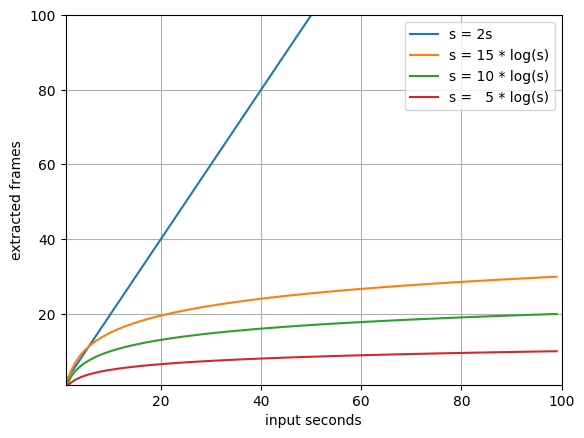
\includegraphics[width=0.5\textwidth]{frame_extr.png}}
    \caption{Comparison of different frame extraction functions.}
    \label{frame_extraction}
\end{figure}

Figure \ref{frame_extraction} shows the growth of the number of frames extracted based on the length 
of the video in seconds, with different values of $k$, compared to the function $n = 2 * s$ that takes one frame each half second. \\
In case of image input, this module is not used. \\
The output of this modue consists in a path to the folder containing the extracted frames and the number of frames extracted.
\subsection{Object detection}
The object detection module detects objects in the frames extracted by the previous module. In case of image input, this module performs the object recognition only on the single image. 
The module uses the YOLOv9 \cite{yolo} model, which is a state-of-the-art and widely used object detection model that can run in short time and provide good results.
The output of this module consists of a list of objects detected in each frame, as well as a set of all objects detected in the batch.

\subsection{Best frame selection}
This module is designed to select the best frame from the ones extracted by the first module. The main reason behind this choise is the computational intensity coming from the frame description module,
that takes $\sim 5-7$ seconds to process a single frame. Thus, passing all the frames would generate a sensitive delay in the process of each video. \\ The extraction of frames is done using FFMPEG \cite{ffmpeg}, a versatile and easy CLI tool that is capable of processing audio and video files. \\
The criterion used to select the best frame has been object of many tests, due to the fact that it is a difficult to generalize task that is highly dependent on the input video. 
Our final proposed solution picks the best frame using a KMedoid algorithm over a latent representation of the images. The latent representation is obtained by passing the image through ResNet18 \cite{resnet}, which is a widely used and efficient image classification model. Since the task is not classification, the ResNet module is used to only get the latent representation of the input, of size $512 \times 16 \times 29 $. The said representation is then reshaped and used to cluster the video and calculate the medoid. In particular, the KMedoid algorithm is used with $k=1$ to get the medoid of the complete. \\
The output of this module is the path and index of the selected frame.  

\subsection{Frame description}
For this crucial task different options of image to text models were evaluated and tested. The main source used for models is the Hugginface text-to-image section\cite{hfaceItt}.  
In the end, the selected model for this task is MoonDream2 \cite{moondream2}, a image-text to text model that is able to produce the answer to a question over the image.
In our case, the used question is \emph{"Describe shortly this image considering it will be used as input to a sound generation model"} that, over different tests, provides good results combined with the following modules.
The choise switched to an image-text to text model since it provides a wider inference than image to text models, that can be used to condition the produced description to better fit our goals.\\
The output of this module is the description of the input image.

\subsection{Prompt enhancer}
The prompt enhancer module is only composed of a single string interpolation that combines the outputs of both the frame description and the object detection modules. An initial option was to combine them using a lightweight Large Language Model, but we decided not to include another model to avoid the increase in computational cost.
The output of this module is the composed prompt, that will be fed in input at the audio generation module. 

\subsection{Audio generation}
The audio generation module feeds the input to the AudioLDM2 model \cite{audioldm2}, which is a state-of-the-art audio generation model that can produce audio from the provided prompt. The model can take as input negative prompts as well, that corresponds to behaviors and keywords we want to avoid. 
This slightly improves the output overall, generating a more enjoyable audio that can better fit the video itself.\\
However, AudioLDM2 has a complex structure that impacts the computational cost of the system. With the available systems, we could not run it on local machines. More details on this can be found in the \textbf{Deployment} section of this report.\\
The output of this module is the output path containing the generated audio.

\subsection{Reconstructor}
The reconstructor module is the final module of the standard pipeline, that produces the output of the system.
It combines the generated audio with the initial input video using FFMPEG \cite{ffmpeg} to produce the final enhanced version of the video. 
The output is the path to the final video, that is served to the user via the Gradio interface.

\section{Deployment}
The deployment of the system is done using Python 3.10.12 on Google Colab \cite{Colab}. The first intention was to whole process run on a local machine, but it quickly became clear that this is not possible due to the high hardware requirements that audio generation models have.
The next idea was to serve the audio generation module over an API, loading it on the machine provided at IST. This hypotesis got aswell discarded for lack of sufficient resources.
\\The Gradio interface is accessed through a public link, which is generated by the library itself. The link is accessible by anyone and can be used to interact with the system.
\\The informations about the used libraries and technologies can be found in the \textbf{Architecture} section of this report.

\section{Implemented features}
At the moment the project is capable of generating music tracks or music and audio tracks with a defined balance between these two audios. It can also produce music or audio and music from an image, with the resulting video lasting for the specified duration. 


\section{Evaluation and benchmarks}
Evaluation of our task has no precise metrcis, since the output is highly subjective that depends on how a music fits on a video or not in a personal opinion.
In our opinion, the resulting audios in our test videos were fitting enough to be considered as a good result.\\
However, we conducted a few tests to assess the time performance of the system. Videos of different time durations have been processed by the system under the same hardware conditions. The required time for the complete process has been recorded, and results are shown in Figure \ref*{time_performance}.

\begin{figure}
    \centerline{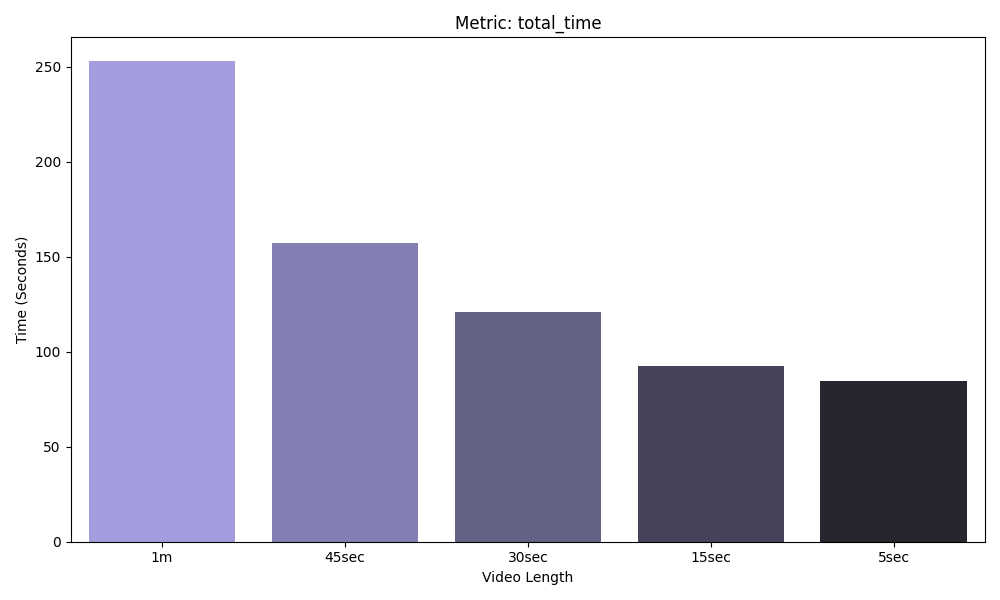
\includegraphics[width=0.5\textwidth]{../Presentation/graphs/total_time.png}}
    \caption{Total time performance of the system.}
    \label{time_performance}
\end{figure}

\section{Conclusions and future work}



\begin{thebibliography}{00}


    \bibitem{chatgptintro}
        \href{https://openai.com/index/chatgpt/}{OpenAI ChatGPT introduction.}

    \bibitem{dall-e}
        \href{https://openai.com/index/dall-e/}{OpenAI DALL-E introduction.}

    \bibitem{ytcopyright}
        \href{https://support.google.com/youtube/answer/6364458?hl=en}{YouTube copyright policies.}

    \bibitem{yolo}
        \href{https://docs.ultralytics.com/models/yolov9/}{Yolov9 documentation} and 
        \href{https://docs.ultralytics.com/models/yolov9/\#citations-and-acknowledgements}{Yolov9 paper reference.}
    
    \bibitem{Colab}
        \href{https://colab.research.google.com/}{Google Colab main page.}

    \bibitem{ffmpeg}
        \href{https://ffmpeg.org}{FFMPEG website.}
    
    \bibitem{resnet}
        \href{https://pytorch.org/vision/main/models/generated/torchvision.models.resnet18.html}{ResNet18 implementation on PyTorch.}
    
    \bibitem{moondream2}
        \href{https://huggingface.co/vikhyatk/moondream2}{MoonDream2 model card on HugginFace.}
    
    \bibitem{Gradio}
        \href{https://www.gradio.app/}{Gradio library main page.}

    \bibitem{hfaceItt} \href{https://huggingface.co/models?pipeline_tag=image-to-text&sort=trending}{HuggingFace image-to-text section.}

    \bibitem{audioldm2} \href{https://audioldm.github.io/audioldm2/}{AudioLDM2 documentation and paper.}
\end{thebibliography}

\end{document}
